\documentclass[10pt,aspectratio=169]{beamer}

\usetheme{metropolis}
\usepackage{amsmath,amssymb,amsfonts}
\usepackage{graphicx}
\usepackage{booktabs}
\usepackage{hyperref}
\usepackage{xcolor}

\graphicspath{{../../figures/hyqad/}}
% No separate section pages

\title{HYQAD: Hybrid AI-Quantum Anomaly Detection for QKD Systems}
\subtitle{Cybersecurity Research Internship --- Progress Report}
\author{Arnav Kapoor}
\institute{CCRI Lab}
\date{July 2026}

\begin{document}

\begin{frame}
  \titlepage
\end{frame}

\begin{frame}{Project Overview \& Objectives}
  \textbf{HYQAD:} Hybrid AI-Quantum anomaly detection framework for Quantum Key Distribution (QKD) systems
  \begin{itemize}
    \item Detect physical-layer attacks (PNS, Detector Blinding, Trojan Horse, Intercept-Resend)
    \item Bayesian GP classifier providing \textbf{calibrated uncertainty} estimates
    \item 3-qubit quantum kernel SVM + quantum-inspired feature engineering (amplitude encoding, MCD covariance)
    \item Sub-10ms edge-deployable inference
  \end{itemize}
  \vfill
  \textbf{Completed:} Framework implementation ($\sim$2000 loc), 5 research articles, 30 unit tests, full benchmark suite
\end{frame}

\begin{frame}{Architecture}
  \begin{figure}
    \centering
    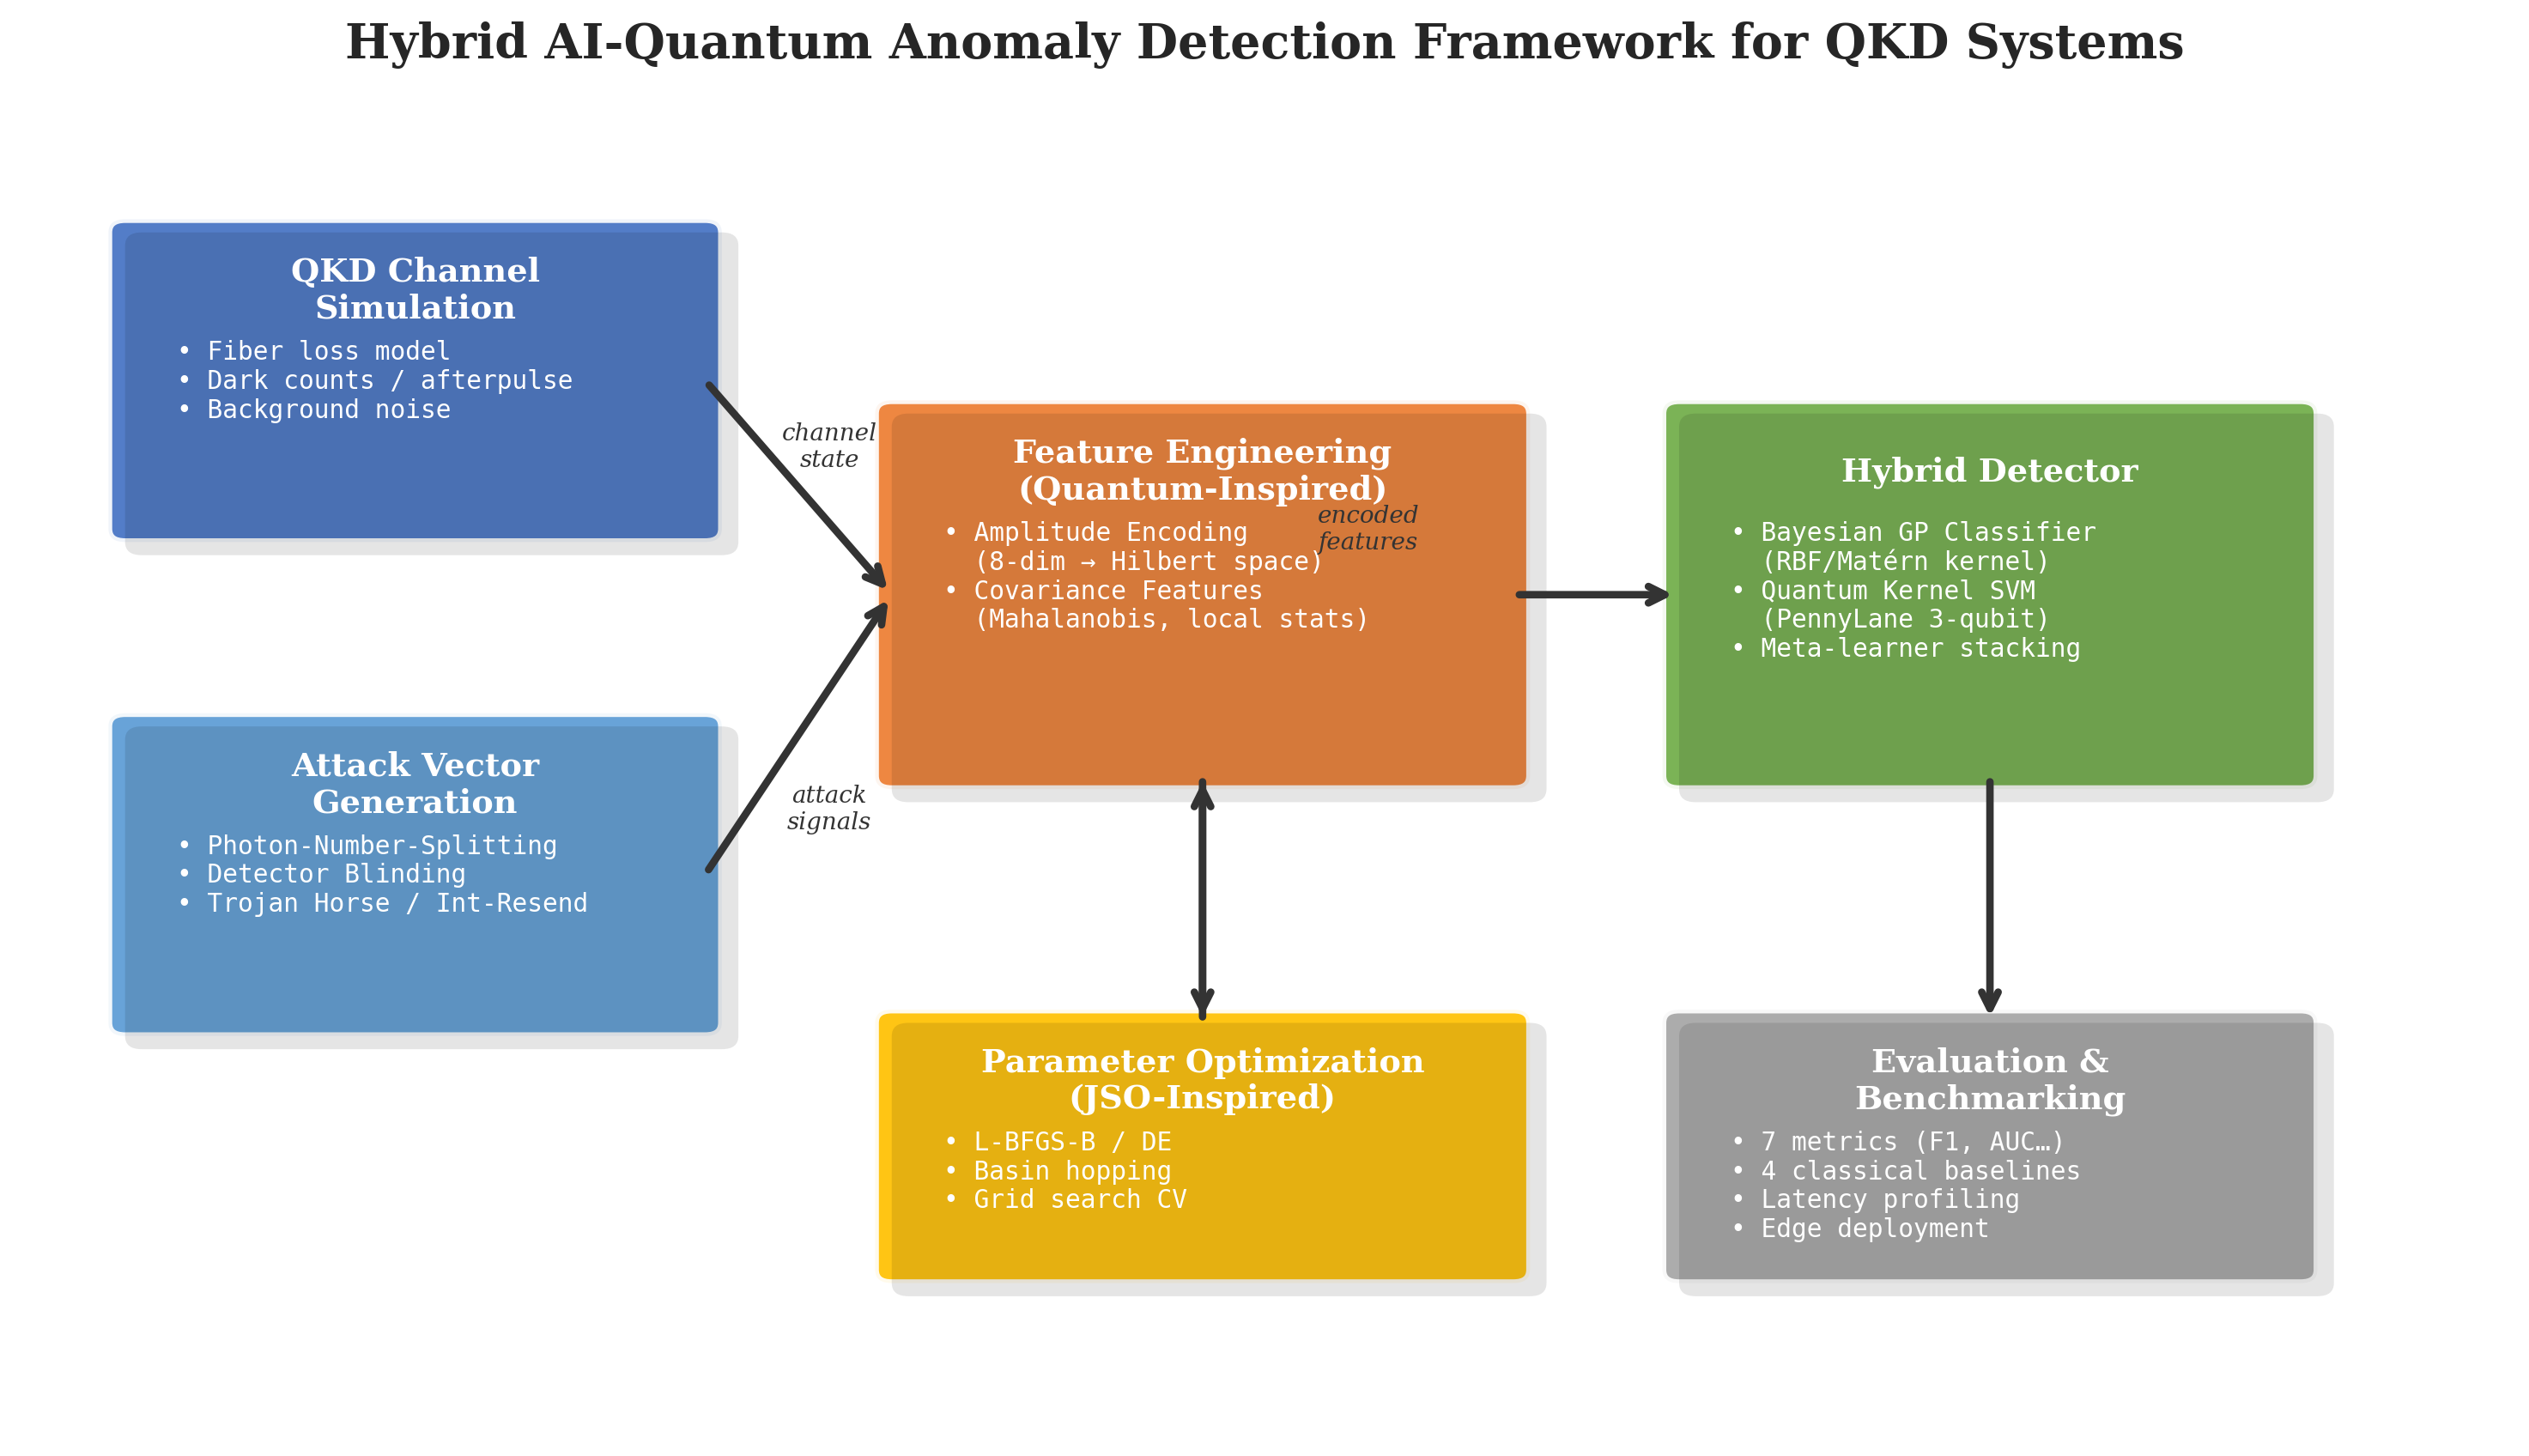
\includegraphics[width=0.7\textwidth,height=0.7\textheight,keepaspectratio]{fig1_framework_hyqad.png}
  \end{figure}
\end{frame}

\begin{frame}{Benchmark Performance (5000 samples, 28-dim features)}
  \begin{table}
    \footnotesize
    \begin{tabular}{lccccc}
      \toprule
      \textbf{Metric} & \textbf{RF} & \textbf{Hybrid} & \textbf{OC-SVM} & \textbf{IF} & \textbf{LOF} \\
      \midrule
      Acc.  & $\mathbf{0.995}$ & 0.940 & 0.894 & 0.748 & 0.755 \\
      F1    & $\mathbf{0.992}$ & 0.889 & 0.810 & 0.269 & 0.302 \\
      AUC   & $\mathbf{1.000}$ & 1.000 & 0.888 & 0.999 & 0.905 \\
      MCC   & $\mathbf{0.987}$ & 0.839 & 0.746 & 0.413 & 0.437 \\
      Spec. & 0.996        & $\mathbf{0.999}$ & 0.958 & 0.594 & 0.628 \\
      \bottomrule
    \end{tabular}
  \end{table}
  \begin{itemize}
    \item RF dominates point estimates; HYQAD uniquely provides \textbf{calibrated uncertainty}
    \item RF near-perfection reflects \textbf{synthetic data difficulty} -- real-world validation needed
  \end{itemize}
\end{frame}

\begin{frame}{Ablation Study \& Key Findings}
  \textbf{Ablation (mean $\pm$ std, 3 seeds):}
  \begin{table}
    \footnotesize
    \begin{tabular}{lcccc}
      \toprule
      \textbf{Metric} & \textbf{RF} & \textbf{GP-only} & \textbf{QK-only} & \textbf{Hybrid} \\
      \midrule
      Acc.  & $\mathbf{1.000}$ & $0.900_{\pm 0.042}$ & $0.700_{\pm 0.000}$ & $0.782_{\pm 0.077}$ \\
      F1    & $\mathbf{1.000}$ & $0.795_{\pm 0.098}$ & $0.000_{\pm 0.000}$ & $0.384_{\pm 0.347}$ \\
      \bottomrule
    \end{tabular}
  \end{table}
  \begin{itemize}
    \item GP drives accuracy; quantum kernel (25 training samples) does not yet contribute positively
    \item $\mathcal{O}(n^2)$ circuit cost limits QK training size -- hardware acceleration needed
  \end{itemize}
  \vfill
  \textbf{Uncertainty calibration:} Rejection-based deferral ($u > 0.4$) raises accuracy to 0.982 (86.3\% coverage)
\end{frame}

\begin{frame}{Latency Profile (Intel i7, CPU)}
  \begin{table}
    \centering
    \footnotesize
    \begin{tabular}{lrr}
      \toprule
      \textbf{Component} & \textbf{Latency (ms)} & \textbf{vs.\ RF} \\
      \midrule
      RF (200 trees) & 0.9 & 1.0$\times$ \\
      Bayesian GP & 5.8 & 6.4$\times$ \\
      Quantum kernel SVM (offline) & 50.0 & 55.6$\times$ \\
      \textbf{Full pipeline (Bayesian)} & \textbf{8.5} & \textbf{9.4$\times$} \\
      \textbf{Bayesian linear est.} & \textbf{0.4} & \textbf{0.4$\times$} \\
      \bottomrule
    \end{tabular}
  \end{table}
  \begin{itemize}
    \item Bayesian linear estimator: 0.4ms -- suitable for real-time edge deployment
    \item Quantum kernel is the bottleneck; approximations (random Fourier features) planned
  \end{itemize}
\end{frame}

\begin{frame}{Challenges \& Planned Work}
  \textbf{Challenges:}
  \begin{itemize}
    \item Quantum kernel latency (50ms/sample on simulator) -- exploring Nystr\"om/random Fourier features
    \item Synthetic data may be too easy (RF AUC = 1.000) -- experimental validation on physical testbeds needed
    \item Attack parameters are modeling assumptions -- need calibration from real QKD hardware data
  \end{itemize}
  \vfill
  \textbf{Planned milestones:}
  \begin{itemize}
    \item[\textbf{Week 3}] Stress-test high-noise regimes, extend attack library
    \item[\textbf{Week 4}] FPGA feasibility study, experimental validation, paper draft
    \item[\textbf{Month 2}] Adaptive GP thresholding, FPGA implementation, real hardware benchmarks
  \end{itemize}
\end{frame}

\begin{frame}{Thank You}
  \centering
  \vfill
  {\huge Questions?}
  \vfill
  \textit{HYQAD: Hybrid AI-Quantum Anomaly Detection for QKD Systems}
\end{frame}

\end{document}
